\chapter{Background}\label{chap:background}
  The main driver to the adoption of Blockchain technology was the ability to solve the double spending problem while maintaining the anonymity and privacy of the transacting user’s information. Double spending is a situation in which a user of a digital currency can spend several times the same amount of money before there has been a realization that the amount has already been spent/claimed.


\section{Blockchain Architecture}
Industry 4.0 applications require careful consideration of security and privacy to prevent unauthorized access or data breaches. Without a strong security system, the system and data are vulnerable to various types of attacks that can compromise data confidentiality and integrity, and disrupt the overall functioning of the system. These attacks include \ac{DDoS}, \ac{ARP} spoofing attacks, data rate alteration, network congestion, manipulation, noise interference, phishing, and config threats. It is crucial to prioritize prevention over reactive defense mechanisms and ensure compliance with legal rules to guarantee confidentiality, integrity, and privacy. The literature suggests that as Industry 4.0 automation increases, so does the risk of new types of cyber-attacks. Therefore, access control, authorization, confidentiality, availability, and integrity are essential concerns in Industry 4.0.

The blockchain technology has the potential to enhance security by eliminating the need for a centralized authority to perform operations. Instead, multiple users participate in verifying and validating transactions. The technology uses a distributed database structure that stores encrypted data from all nodes and verifies them using checks like \ac{MHT} and \ac{ECC}. Although there is a risk of database crashes or corruption, the linking of transactions using cryptographic keys and immutable ledgers makes it challenging for attackers to manipulate or delete information. Timestamps, public audit, and consensus mechanisms ensure data is stored in an immutable manner. The use of these mechanisms makes the security architecture robust and ensures data integrity and privacy.

\subsection{Merkle Hash Tree}

Ralph Merkle is the namesake of Merkle trees \cite{merkle_digital_signature}, which are utilized in cryptocurrencies like Bitcoin to efficiently and securely encode and encrypt blockchain data. These trees are also known as hash trees and are created through a process of repeatedly hashing pairs of nodes until only one hash, known as the root hash or Merkle root, remains. The construction of Merkle trees is done using a bottom-up approach. Each transaction is hashed, and then each pair of transactions is concatenated and hashed together, continuing until there is only one hash for the entire block. Figure \ref{fig:Simple binary hash tree.} shows a simple binary Merkle tree.

 \begin{figure}[H]
 \centering
  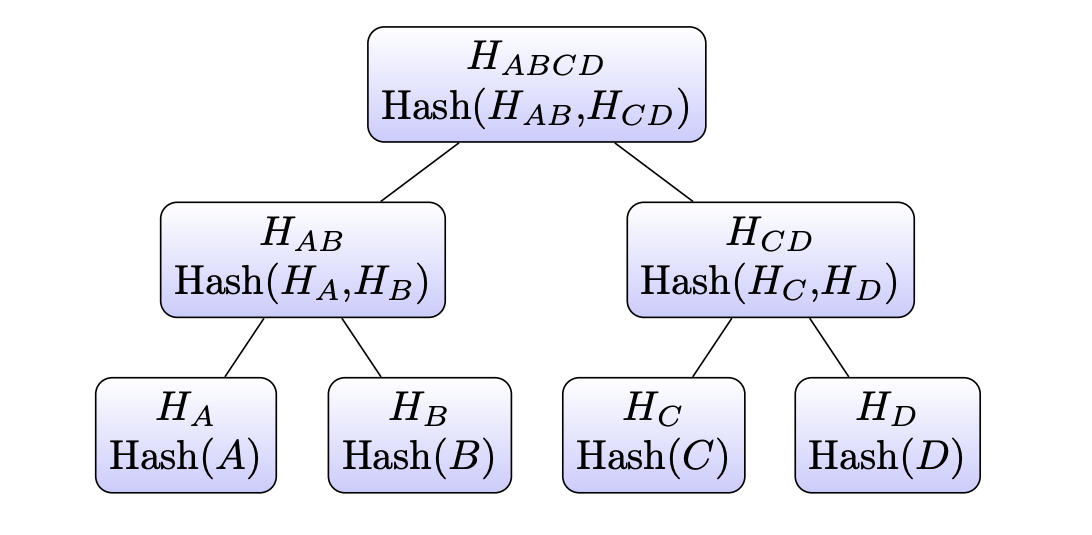
\includegraphics[width=0.8\textwidth]{simple binary hash tree.png}
  \caption{Simple binary hash tree.}
  \label{fig:Simple binary hash tree.}
\end{figure}

The Merkle tree allows us to efficiently prove that some piece of data was used to generate a root hash without needing to have access or store all the original pieces of information. The proof size (Merkle proof) scales logarithmically with the number of data blocks as opposed to simply concatenating and hashing all the data at once, which would require storing large amounts of data. For example, in Figure \ref{fig:Simple binary hash tree.}, if we wanted to check if the piece of data A was used to generate the root hash, we would only need \ac{HB} and \ac{HCD}, because the latter summarizes data C and D. If any of the data changes, the root hash will also change. This may be extended to also authenticate large databases of potentially unbounded size by all computers large and small, without compromising on scalability and avoiding centralization of the services.

\subsection{Elliptic Curve Cryptography}

Victor Miller and Neal Koblitz independently introduced the concept of elliptic curve ciphers in the mid-1980s. These ciphers work similarly to other public-key cryptosystems, but they use operations on elliptic curves instead of modular arithmetic. The security of \ac{ECC}, like all public-key cryptosystems, depends on difficult mathematical problems. One such problem is the elliptic curve discrete logarithm problem, which involves finding an integer k given two points G and Y on an elliptic curve such that Y = kG (i.e., Y is G added to itself k times). Currently, methods for calculating discrete logarithms of elliptic curves are much less efficient than traditional methods of factoring or calculating discrete logarithms.

\subsubsection{Example}

We consider here that the secret keys $KA$ and $KB$ are generated randomly by sender (A) and receiver (B). Therefore, the randomly generated keys $KA$ and $KB$ are given by:

\begin{flushleft}
$KA = 1b66c808e6b5be6d6620934bc6ff
a2b8b47f9786c002bfb06d53a0c27535641a5d1$
\end{flushleft}

\begin{flushleft}
    

    
$KB = 1c7d15195432d1ac7f38aeb$
$054d07d9b2e1faa913b7d08a4d5efdd4a1ee8d9a31916d53a0c275356
41a5d0d1$
\end{flushleft}

Let us assume that (A) and (B) pre-agreed with the point $Q$ given by:

\begin{equation*}
\begin{split}
Q = (&0xd458e7d127ae671b0c330266d246769353a012073e97acf8, \\
&0x3259305sfgr211f446bddc050cf7fb11b5673a1645086df3b)
\end{split}
\end{equation*}
  

When (A) sends the point $X = KAQ$ to (B) and (B) shares the point $Y = KBQ$ with (A), then the generated secret key is shared between (A) and (B). This secret key is common for both users and is given by:

$KS = 0x94f5a1cf2ed1dbb4322178df6bb4dd742c541884618b2989a3e5e66319667a640$

The elliptic curve which is being used for the \ac{ECDH} calculations is a 256-bit named curve brainpoolP256r1 (which uses a Diophantine equation for the generation of points). The private keys are randomly 256-bit (64 hexadecimal digits). The public keys and shared keys are 257 bits (65 hexadecimal digits, 256 bits due to key compression). Due to randomization, the secret keys $KA$ and $KB$ are different, but the calculated shared secret key between (A) and (B) will always be the same.

\section{Double Spending Problem}

The primary motivation for the acceptance of Blockchain technology was its capability to resolve the issue of double spending without compromising the confidentiality and privacy of user information during transactions. Double spending refers to the circumstance where a digital currency user can spend the same amount of money multiple times before it is detected that the amount has already been utilized or claimed.
\subsection{Illustration}

Problem starts with when user requests a transaction , miner picks the transaction and solve complicated problem to add block to blockchain as long as miner spends all his currency and sends this information to the real blockchain but not to his own isolated chain.Then, the corrupted miner solve problem faster than real miners (they are needed to verify the block and add it to blockchain) and he make an isolated blockchain bigger than the real one. 
As a result, the democratic governance rule states that the blocks will add to the larger one by removing the previous records that they have ,so in the new isolated chain, the corrupted miner would be able to spend all of the currencies that he had spent once in the real blockchain.

\subsection{Examples}
As for Table \ref{tab:Examples of attacks to blockchain}, Blockchain networks are not completely immune to attacks, with common examples including Wallet Attacks, Double Spending Attacks, \ac{DDoS} Attacks, \ac{BGP} Hijacking, Spam Attacks, \ac{DAO} Attacks, and Selfish Mining Attacks. These attacks can result in theft of funds or disruption of network operations. To mitigate these threats, blockchain networks use security measures such as encryption, multi-factor authentication, and consensus algorithms, but continuous monitoring and updates are necessary to ensure network and user protection.
\begin{table}[ht]
\caption{Examples of attacks to blockchain}
\resizebox{\textwidth}{!}{%
\begin{tabular}{|l|l|l|l|l|}
\hline
No & Attack Name & Targeted  Area & Effect of Attack & Possible   Countermeasure found \\ \hline
1. & Brute Force Attack & \begin{tabular}[c]{@{}l@{}}Computing  Power,\\    \\ Pow Consensus\end{tabular} & Data encryption & inserting observers in the   network, notify the merchant about an ongoing double spend \\ \hline
2. & Refund Attack & Payment protocol & Lose money, reputation & publicly verifiable evidence \\ \hline
3. & Wallet Attack & Private key & Lose of bitcoin & threshold signature based   two-factor security, hardware wallets , Password-Protected Secret Sharing   (PPSS) \\ \hline
4. & \begin{tabular}[c]{@{}l@{}}Time      Hijacking\\    \\ Attack\end{tabular} & Network & Fake peers & constraint tolerance ranges,   network time protocol (NTP) or time sampling on the values received from   trusted peers \\ \hline
5. & Long Range Attack & Database[ & Alter transaction history & Nodes trust identity provider,   implementation of trusted hardware \\ \hline
6. & BGP Hijacking & Database, Protocol & Fake transaction & Human driven process consisting   of altering configuration or disconnecting the attacker. \\ \hline
7. & Sybil Attack & Network & \begin{tabular}[c]{@{}l@{}}Pseudonymous     identities,\\    \\ threatens user privacy\end{tabular} & Xim (a two-party mixing protocol) \\ \hline
8. & DDOS Attack & Network & \begin{tabular}[c]{@{}l@{}}Generates      huge                  unnecessary\\    \\ responses about transaction\end{tabular} & Proof-of-Activity (PoA) protocol \\ \hline
9. & Eclipse Attack & Network & inconsistent view of the   network and blockchain & Use whitelists, disabling incoming   connections \\ \hline
10. & DAO Attack & Computing Power & Fake transaction & Hard fork proposal, Soft fork   proposal \\ \hline
11. & \begin{tabular}[c]{@{}l@{}}Nothing     at                 Stake\\    \\ Attack\end{tabular} & Block & Slow consensus time & Slasher Protocol \\ \hline
12. & Pool Mining Attack & \begin{tabular}[c]{@{}l@{}}Block,    Computing\\    \\ Power\end{tabular} & Slow          verification                   time,            fake transaction & Not Found \\ \hline
13. & \begin{tabular}[c]{@{}l@{}}Double  Spending\\    \\ Attack\end{tabular} & Bitcoin                   transaction, Pow    Consensus & lose products, create forks & Recipient oriented transaction \\ \hline
14. & \begin{tabular}[c]{@{}l@{}}Selfish       Mining\\    \\ Attack\end{tabular} & Block,                   Computing power & Increase    personal    share                    on transaction & Address bitcoin protocol and   raise threshold, computing branches are same length and propagate all of   them, Zero Block technique \\ \hline
\end{tabular}%
}
 
  \label{tab:Examples of attacks to blockchain}
\end{table}

One common attack is the \ac{Wallet}, which involves hacking into a user's wallet and stealing their private keys. Once the attacker has access to the private keys, they can easily transfer the funds to their own wallet. \ac{Double Spending} Attack is another popular attack where the attacker attempts to spend the same coins twice, causing a loss of funds to the network.

\ac{DDoS} Attack is also a potential threat to blockchain networks. This attack aims to overload the network with a large volume of traffic, which can cause the network to become slow or even unresponsive. \ac{BGP} Hijacking is another type of attack where attackers redirect the network's traffic to a malicious server in order to carry out their nefarious activities.

\ac{Spam} Attack is another attack where attackers send a large number of transactions to the network in order to overload the network's capacity. The \ac{DAO} Attack is a sophisticated type of attack that occurred in 2016, which involved exploiting a vulnerability in a smart contract. This attack resulted in the loss of millions of dollars worth of cryptocurrency.

Finally, \ac{Selfish Mining} Attack is a type of attack where a group of miners try to monopolize the mining process by withholding the blocks they have mined from the network and publishing them later. This allows them to gain an unfair advantage over other miners and can lead to centralization of the network.

\subsection{Double Spending Probelm Solutions} 
 Smart contract applications are similar to web applications that run over the blockchain. Like web application bugs, they also comprise errors, however, these bugs can lead to serious challenges. For example, the \ac{DAO} was able to raise 150m whilst the attacker was able to steal about 60m due to code bugs. Rubixi and GovernMental are some of the smart contract applications which had flaws due to code bugs. Application bugs may not only allow attackers to steal money, but also influence an application to function differently.
\begin{itemize}
  \item Mythril

Mythril is a tool used to enhance the security of smart contracts written in Solidity by detecting any potential errors in the code. As an open-source tool, Mythril employs symbolic execution technique to identify potential security vulnerabilities. To analyze security flaws, Mythril executes smart contract bytecode in a specialized \ac{EVM} and employs four significant stages to achieve its security analysis. In the event that a program flaw is discovered, Mythril conducts an analysis of input transactions to establish the possible reasons behind the flaw. This security approach assists in identifying the underlying cause of the program's vulnerability, and as a result, reducing the likelihood of its exploitation. Additionally, if a developer provides the source code of the contract, Mythril is capable of locating and identifying any bugs in the code.


Mythril is an excellent tool for analyzing smart contracts built for \ac{EVM} bytecode. It can detect security vulnerabilities in Ethereum, Hedera, Vechain, Tron, Quorom, Roostock and basically every or any \ac{EVM} compatible blockchains. Mythril is exclusively based on symbolic execution engine. It thoroughly goes through all probable states within a contract with the help of function(s) call. Mythril analysis uses the bytecode of the smart contract to decompile it back into \ac{EVM} opcode instructions. It then explores all probable program states over ‘n’ transactions. Mythril uses LASER, \ac{SVM} to create an environment, where it executes opcode and reveal vulnerabilities. LASER computes all probable program states. Mythril uses a number of analysis modules to determine if the vulnerability subsists. If a compromised or vulnerable state subsists. Mythril uses Z3, an automated theorem prover, to prove or disprove the extendibility of the state. Z3 is delivered by Microsoft Research under \ac{MIT} license. All the issues about symbolic execution engines, detecting vulnerabilities are well documented.

\begin{itemsize}
   \item[--] { Mythril installation / Usage}
   
a.	Environment preparation by installing Homebrew, python and python3.

b.	Install Mythril using following commands from Figure \ref{fig:commands}.

 \begin{figure}[H]
 \centering
  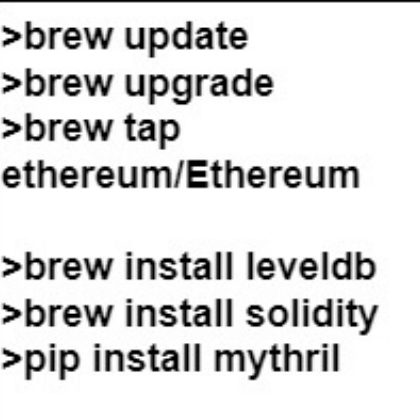
\includegraphics[width=0.3\textwidth]{commands.png}
  \caption{Mythril Installation commands}
  \label{fig:commands}
\end{figure}

c.	Checking Mythril for proper running >myth -x smartcontract.sol`.

\end{itemsize}

\hfill
\item	ZEUS

ZEUS ensures both reliability and scalability by using three main observations. Firstly, even though the blockchain operates like a concurrent system with task-based semantics, a transaction consists of only one call chain that starts from a publicly visible function in the smart contract. This means that verifying most properties requires exploring a much smaller state space. Secondly, smart contracts are driven by both control and data. Therefore, ZEUS models contracts using abstract interpretation, which computes loop and function summaries over data domains. These summaries are used during the model checking phase, which operates on a reduced state space. Lastly, \ac{CHC}s are used to represent verification conditions, which can be easily solved by \ac{SMT} solvers.


\hfill
\begin{itemize}

    \item[--] Implementation
    

In order to develop a tool for translating Solidity smart contracts to \ac{LLVM} bitcode and detecting bugs, we utilized the  of the smart contract derived from the Solidity compiler solc, and implemented both the policy builder and the translator in C++. The policy builder required approximately 500 lines of code, while the ranslator, including the \ac{LLVM} passes for bug detection, required approximately 3000 lines of code.

    \hfill

For ease of implementation, we leverage Seahorn as our symbolic model checking backend for verification of policies. Instead of building the verifier from scratch, we determined that Seahorn provides us with an off-the-shelf implementation of generating 	verification conditions using \ac{CHC}s over \ac{LLVM} bitcode. Furthermore, use of existing tools that have been tested for bugs and fine tuned for performance, both of which are critical for verifiers, helps reduce ZEUS’s false alarms and improve verification times. However, as will be shown later in § VI-D, ZEUS is not tied to Seahorn; it can be used with any other verifier that operates upon \ac{LLVM} bitcode, such as SMACK or DIVINE .
\end{itemize}

\item Blockchain-Based Sybil Attack Detection

As shown in Figure \ref{fig:sybil detection model} ,In order for a sensor node to join the network, it must request access from the \ac{CH} and provide its unique ID. Once granted access, the sensor node will periodically update its cluster membership information to account for any changes in its position or range. The \ac{CH} will use a trust management model to evaluate the trustworthiness of each sensor node and generate a transaction containing the node's ID, location, and trust value for addition to the blockchain. If a sensor node relocates to a new cluster, it must request access again, and the corresponding \ac{CH} will check the blockchain for previous information on the node. Each \ac{CH} includes a timestamp for each period to detect any Sybil nodes. If a node is found to be a Sybil node, it is considered malicious and denied access. Otherwise, it is considered legitimate.
	 

 \begin{figure}[H]
 \centering
  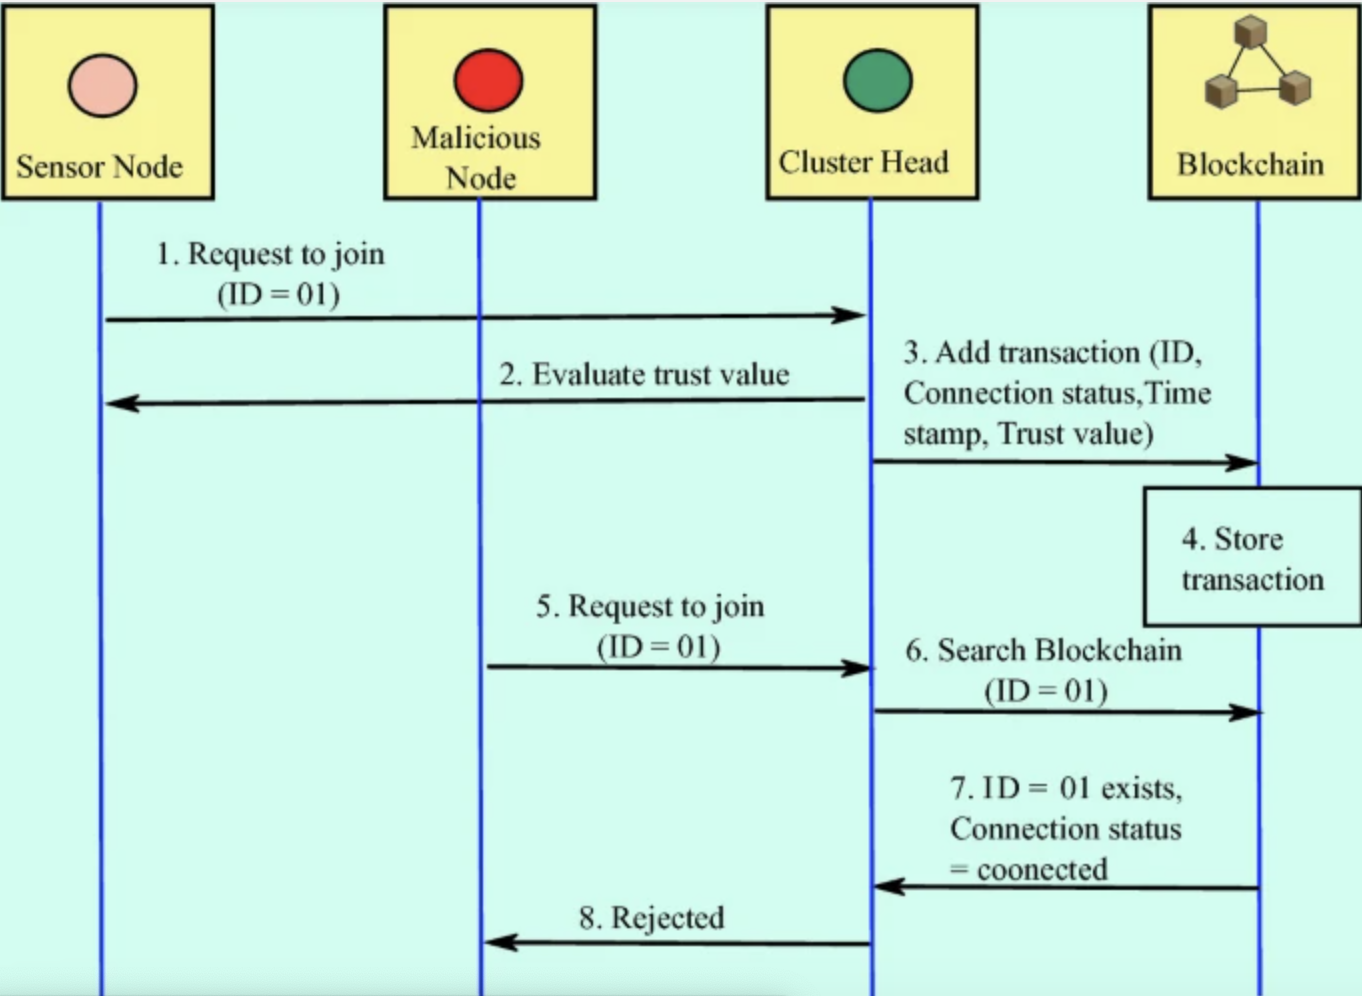
\includegraphics[width=0.5\textwidth]{sybil detection model.png}
  \caption{Blockchain-Based sybil detection model}
  \label{fig:sybil detection model}
\end{figure}
\begin{itemize}
    \item Trust model 
To estimate the trustworthiness of sensor nodes in the dynamic underwater channel, a\ac{HMM} is employed. The \ac{HMM} is capable of handling the changing nature of the network. The \ac{HMM} considers packet loss and errors as observable states, while trustworthiness and maliciousness are hidden states. By analyzing the observable states, the \ac{HMM} can effectively determine the level of trust or distrust associated with each sensor node.
\end{itemize}

\item Pikachu Protocol(LRA)

As Bitcoin does not allow for stateful smart contracts, we use an aggregated public key to represent the configuration of validators Ci in the \ac{PoS} system. When the set changes significantly enough to configuration Ci+1, the aggregated key must be updated in the Bitcoin blockchain. This is done by having a transaction transferring the funds associated with the aggregated key of the previous validators Ci to the new aggregated key controlled by validators in configuration Ci+1. Instead of having each validator in Ci send a transaction to the Bitcoin network, this transaction is signed interactively, off-chain, and all the signatures are aggregated into one constant-size signature. Furthermore, we store the Merkle root of the state of the checkpointed \ac{PoS} blockchain in the Bitcoin OP-RETURN field of the transaction from Ci to Ci+1. We store the data pertaining to this checkpoint off Bitcoin blockchain. While the data pertaining to the checkpoint could be stored anywhere (e.g., IPFS \cite{protocollabs_ipfs}) and validated against the state root stored in the Bitcoin transaction — our implementation uses a content-addressable key-value store implemented on top of the \ac{PoS} system to store the actual checkpointed state. Figure \ref{fig:Pikatchu protocol model} illustrates the high-level protocol. We note that since our work is based on Schnorr threshold signatures and uses Bitcoin’s Taproot, it could be of independent interest to any project looking to implement threshold signing transactions on Bitcoin (for example, sidechains \cite{bell_proof-of-stake}).


 \begin{figure}[H]
 \centering
  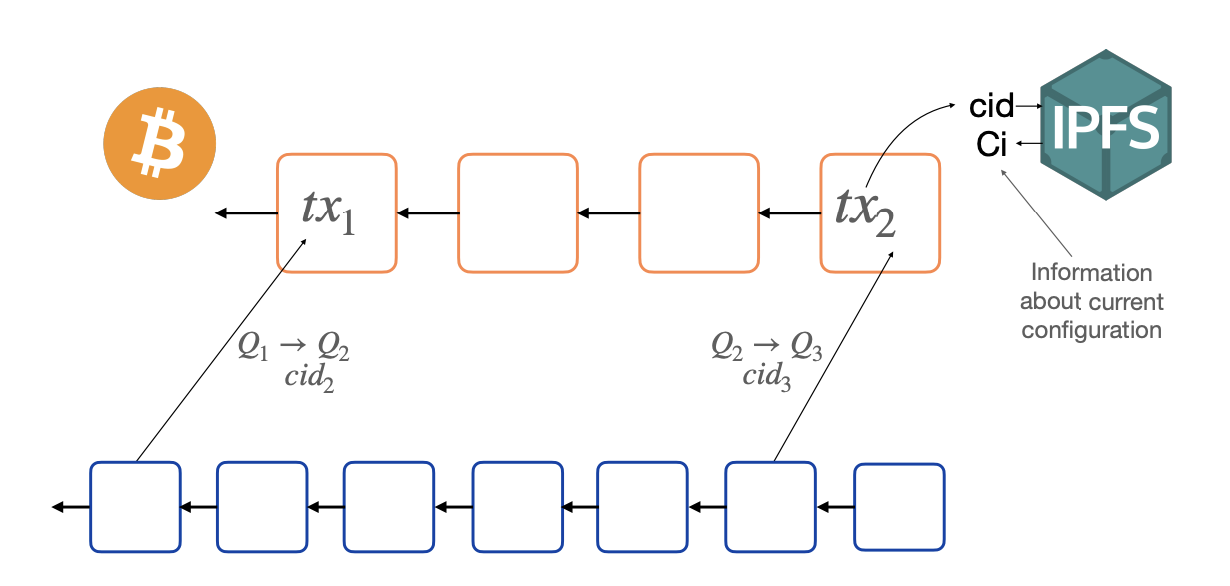
\includegraphics[width=0.5\textwidth]{pikatchu.png}
  \caption{Pikatchu protocol model}
  \label{fig:Pikatchu protocol model}
\end{figure}
\end{itemize}

\section{Applications of Blockchain}

Blockchain technology has come a long way since its inception as the underlying technology for Bitcoin. Today, it has found applications across various industries, ranging from finance to healthcare, logistics to energy, and more. Blockchain's ability to provide decentralized, transparent, and immutable records make it a promising solution for industries looking to improve their operations and increase efficiency.

In finance, blockchain is being used for digital identity verification, cross-border payments, and to enable faster and more secure settlements. Healthcare is another industry that can benefit from blockchain's tamper-proof record-keeping and secure sharing of medical data among healthcare providers. In logistics, blockchain can help in supply chain management, by providing a transparent and secure record of goods as they move across various stages of the supply chain.

Energy is yet another industry where blockchain is being explored for its potential to enable a more efficient and decentralized energy system. Blockchain can facilitate peer-to-peer energy trading, where energy producers can sell their excess energy to consumers directly, bypassing the need for intermediaries.

These are just a few examples of the many applications of blockchain technology as shown in Figure \ref{fig:Blockchain applications}. With its potential to increase transparency, reduce fraud, and lower costs, blockchain is likely to continue to disrupt industries and create new opportunities for innovation.

 \begin{figure}[H]
 \centering
  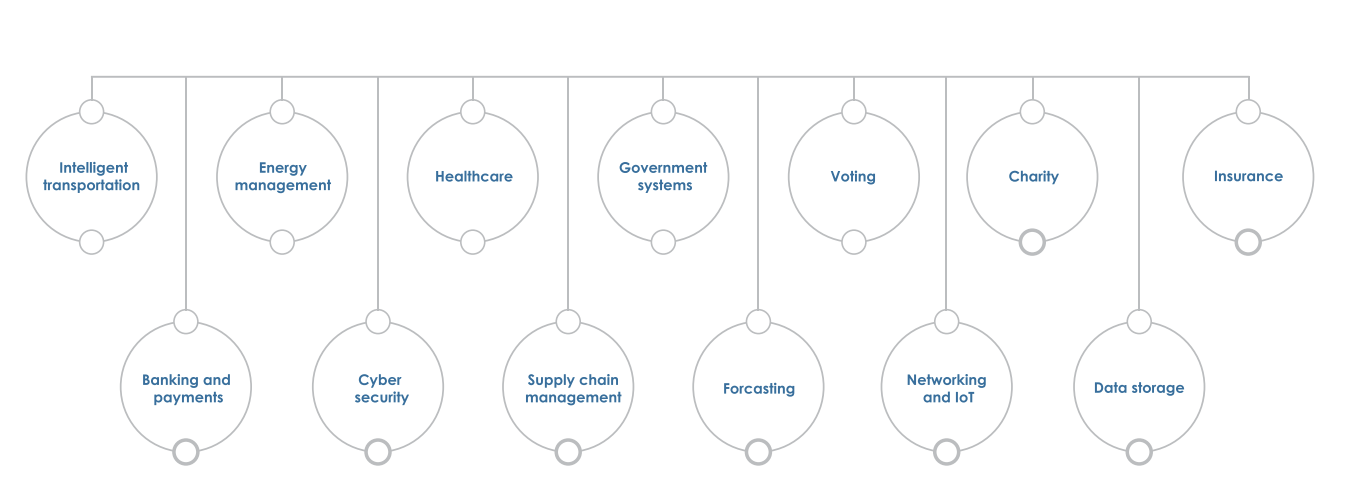
\includegraphics[width=0.8\textwidth]{blockchain applications.png}
   \caption{Blockchain applications}
  \label{fig:Blockchain applications}
\end{figure}
One of the most promising applications of blockchain technology is in the realm of financial services. Blockchain-based platforms have the potential to revolutionize traditional banking by providing faster, cheaper, and more secure transactions. It can also enable new types of financial services, such as peer-to-peer lending, microfinance, and remittances.
Another area where blockchain technology can make a significant impact is supply chain management. By using a blockchain-based platform, it is possible to track goods from their origin to their destination, ensuring transparency and reducing the risk of fraud. This can improve efficiency, reduce costs, and increase trust between parties.
Blockchain technology can also be used in voting systems to enhance transparency, security, and verifiability. By using a blockchain-based platform, it is possible to prevent tampering, ensure anonymity, and allow for the secure storage and retrieval of votes.
Other potential applications of blockchain technology include identity management, healthcare, real estate, gaming, and energy management. Overall, the potential applications of blockchain technology are vast, and it is likely that we will see more innovative use cases emerge in the future.

\subsection{Blockchain in Transportation}

The \ac{BCTLF} is an intelligent framework for transportation and logistics that uses blockchain and \ac{IoT} technology. Unlike traditional vehicular communication systems, which are susceptible to privacy breaches that compromise the security of messages containing sensitive information such as the identity of the driver, type of vehicle, and location, the \ac{BCTLF} offers a solution. To address this issue, a common approach has been to use pseudonyms to conceal the data. However, studies have shown that the expense of maintaining these pseudonyms can escalate, and distributing certificates can be challenging.


Smart vehicles and electric cars are equipped with advanced technology including embedded computers, GPS systems, short-range wireless network interfaces, and access to in-car sensors and the internet. To ensure that sensitive data such as driver and vehicle identity, cryptographic keys, location, predicted travel direction, traffic and road congestion is shared and stored safely, a secure implementation of sharing and storing must be established. This requires a fully or semi-distributed vehicular network topology to avoid security vulnerabilities and bottleneck issues that may arise in centralized systems. The use of blockchain technology can be beneficial in managing data in the \ac{IoV} processing layer and security layer, which can lead to innovative traffic services and secure data transfer while protecting vehicular systems from security attacks.

As an application example, a simple selection mechanism of the charging unit for \ac{EV} drivers is developed based on smart contracts. a scheduling approach for \ac{EV} charging was proposed considering the battery capacity, the rate or behavior of charging and discharging operations, and the relative cost of charging. This mechanism could be extended to consider other selection criteria, such as actual battery status, traffic congestion, and service delay. Other research works focused on designing efficient energy trading frameworks for \ac{EV}s. In \cite{jabbar2022blockchain}, an optimized cost-aware trading energy platform was studied over a consortium Blockchain. This platform applied a contract-based incentive mechanism to respect the preferences of \ac{EV}s and improve their participation cycle.

The payment research field concentrates on investigating new and advanced payment and billing solutions for users of the \ac{IoV}. These solutions are aimed at ensuring secure and efficient transactions while also optimizing energy consumption and pricing. In the \ac{IoV} processing layer, there is a suggestion for a Blockchain-based billing service that guarantees secure transactions between electric vehicles \ac{EV}s and charging stations. Similarly, a different study recommends a unique transaction structure for Hyperledger systems that allows for trustworthy and tamper-proof payments. Moreover, researchers have developed an optimization model for the distributed scheduling mechanism of \ac{EV} battery swap stations, which helps to decrease power generation cost and load. In the \ac{IoV} communication layer, a new configuration of \ac{EV}s and charging stations has been created to personalize Bitcoin transactions in a private network, which leads to reduced costs and verification delay.
 
\subsection{Blockchain Role in Climate Change }
In recent times, global warming has become an increasingly urgent issue, and its impacts are being felt in many countries. The primary cause of this phenomenon is human-generated greenhouse gas emissions, which could result in an increase of 2.8◦ by 2050 if no corrective measures are taken in the current decade. blockchain technology could play a role in addressing this issue by limiting human activity. Deforestation, caused by factors such as factory and livestock farming, results in reduced CO2 absorption and the buildup of CO2 in the atmosphere. Blockchain technology can reduce paperwork and streamline digital applications, thus minimizing human activities that contribute to this problem. By implementing blockchain by 2030, global warming could potentially be reduced by at least 4◦ by 2050. Additionally, the authors identified several limitations of the \ac{REDD+} project and proposed solutions based on blockchain technology, such as cryptocarbon management, green finance, and sustainable investments.

There are many climate-conscious blockchain initiatives in various stages of development. SolarCoin, for example, uses a blockchain platform to incentivize solar-energy producers by rewarding every megawatt-hour of electricity they produce with one free SolarCoin. This digital reward can be used as a medium of exchange or converted to any other currency. Projects such as Earth Dollar aim to link carbon credits (pollution permits that are issued for emissions avoided elsewhere) to blockchain tokens (representations of a particular asset or utility within the platform). Some initiatives are enabling automated smart-contract payment protocols, so that embodied carbon emissions from consumer purchases can be calculated and carbon credits purchased automatically. Infinite Earth’s Veridium Labs, for example, a HongKong-based private company working in partnership with IBM, are connecting their payment system (VerdePay) with carbon credits produced from Infinite Earth’s Forest reserve in Rimba Raya, Central Kalimantan.

\subsection{Blockchain and Health Care}

Blockchain technology can be utilized effectively in the healthcare industry to store sensitive patient data such as medical records, images, videos, and documents. These data require high levels of security and privacy while also being readily available to authorized users. By implementing blockchain, the security and privacy of data can be maintained. A healthcare model based on Bitcoin can store health data from individual users, but the storage management system is not bandwidth-intensive, and network resources are dispersed through throughput optimization. A better solution is to use an access control manager and store instances in a database management system. Authorized administrators can access the encrypted and time-stamped records using a unique identifier that locates them in the storage device. All the data stored in the blockchain database are referred to as data lakes, which are crucial for data.


Blockchain technology has gained popularity in healthcare, especially in the \ac{EMRs}. \ac{EMRs}, also known as \ac{EHRs} or \ac{PHRs}, refer to patients' medical or health-related data that are electronically created, stored, and managed. A significant amount of research has been devoted to the use case of blockchain in managing \ac{EMRs}, with almost half of the selected papers (32 out of 65) addressing this topic. The decentralization, immutability, data provenance, reliability, robustness, smart contracts, security, and privacy features of blockchain are being highlighted as reasons why it is suitable for storing and managing \ac{EMRs}. Some studies are focused on facilitating patient-centric data sharing among various healthcare stakeholders, such as providers, researchers, and insurers. In line with the European  \ac{GDPR}, which requires explicit consent from patients for the processing of sensitive personal data, blockchain is widely proposed as a technology that can empower patients to control how their data are shared, processed, or used within the healthcare platform.


 Figure \ref{fig:Enablers of blockchain implementation in healthcare services} illustrates the several on-ground industrial representatives of
Blockchain capabilities to successfully implement healthcare culture perspectives and overall development. There have been various associated industrial/medical-care supporters or providers, which helps carry out the research and investigations for realising the Blockchain practices in healthcare and its core domains, too \cite{nguyen2018}\cite{kumar2020}. These observed pro
viders BurstIQ, Guardtime, Robomed, Simply vital, Encrypgen, Chronicled, Tieion, etc., are the few agencies supplying and favouring the
practising of Blockchain technology at ground levels.


 \begin{figure}[H]
 \centering
  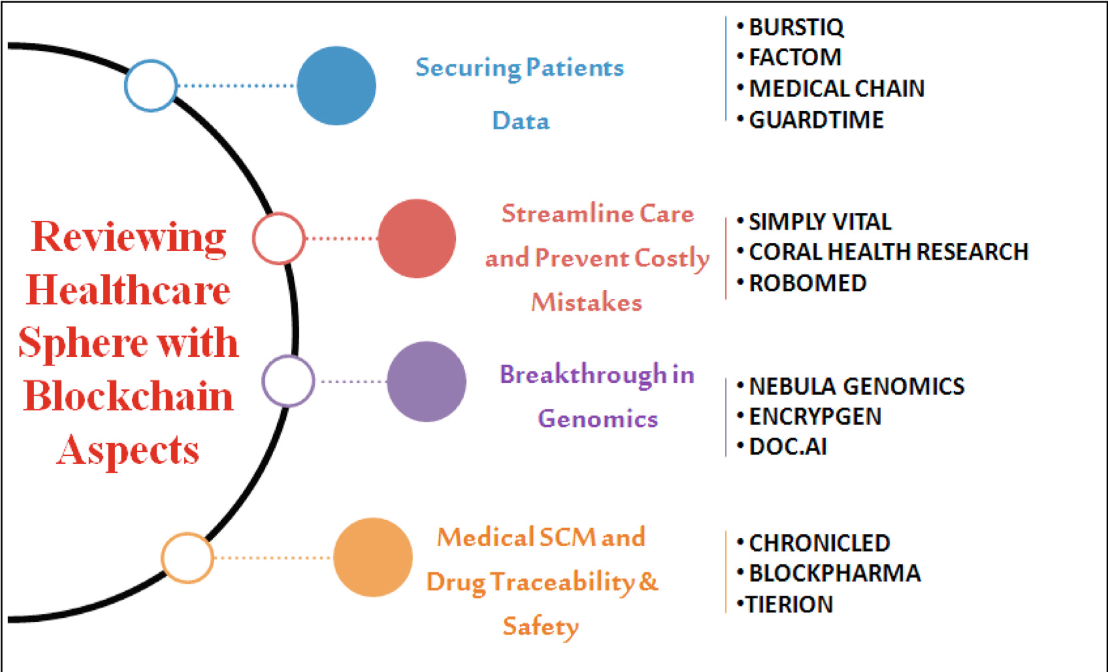
\includegraphics[width=0.8\textwidth]{enablers of blockchain.png}
  \caption{Enablers of blockchain implementation in healthcare services.}
  \label{fig:Enablers of blockchain implementation in healthcare services}
\end{figure}

Guardtime, a company that utilizes a blockchain-powered platform to ensure the security of more than 1 million patient records in Estonia, is recognized in various reviews as a prominent example of blockchain implementation in \ac{EMRs} management \cite{angraal2017blockchain}\cite{mettler2016blockchain}. Another notable illustration is the MedRec project \cite{azaria2016medrec}, jointly developed by \ac{MIT} Media Lab and Beth Israel Deaconess Medical Center. This project aims to empower patients by granting them control over their own data, allowing them to determine who can access it through fine-grained access permissions built on the blockchain. Additionally, the \ac{GHN}, developed by the US startup Gem on the Ethereum blockchain platform, enables different healthcare practitioners to have shared access to the same data \cite{azaria2016medrec}. Healthbank, a Swiss digital health company, is also actively engaged in empowering patients to have complete control over their data using blockchain technology \cite{azaria2016medrec}. In another publication \cite{engelhardt2017hitching}, the author discusses the Medicalchain project, which utilizes a blockchain-based platform to facilitate the sharing of patients' medical records across international healthcare institutions. The author also mentions the Healthcoin initiative, which aims to construct a global \ac{EMRs} system. Various other entities such as Factom, HealthCombix, Patientory, SimplyVital, IBM's Watson, BurstIQ, Bowhead, QBRICS, and Nuco are actively involved in different initiatives and projects that leverage blockchain for patient-centric \ac{EMRs} systems \cite{engelhardt2017hitching}.


\section{Smart Contracts}

Smart contract technology is a digital transaction protocol that operates on its own to enforce the conditions of a contract and establish an understanding between multiple parties. Smart contracts are characterized by their disintermediation and transparency, which facilitate commercial efficiency, decrease legal and transaction costs, and enable anonymous transactions. Their many advantages make them a highly sought-after technology, particularly in the financial industry where they minimize the risk of non-payment and fraud while enhancing the quality of financial contracts with a level of trust that is independent of intermediaries.

Although technology supporting smart contracts has seen numerous advancements,their application in various companies remains poorly understood. Businesses are facing new challenges concerning system security and information technology, as well as trust in data transaction systems and transparency in data exchange between different organizations. The decentralization of business processes and workflow within organizations poses a further challenge in meeting the technological requirements of companies that aim to standardize data transaction security, trust, and transparency. To address these organizational data transaction issues, smart contract technology based on blockchain is suggested as a potential solution for companies.

\subsection{Principal of Operation}
According to \cite{kemmoe_recent_2020}, we introduce a high-level overview of a smart
contract’s process, starting from its development until the
verification of transactions. Figure \ref{fig:Overview of smart contracts} provides a graphic representation of those different steps.
Before diving into the smart contract’s process, we give a
definition of the different terms that will be used:
\begin{itemize}
    \item  Developer: an individual who implements the logic of a
smart contract using a specific set of instructions compatible with or provided by a blockchain platform
    \item  User: any entity that uses the services of a smart contract
    \item Transaction: a query made to a smart contract program
    \item Blockchain platform: the set of applications and protocols used to maintain and manage a blockchain
    \item Node: an entity having an account on the blockchain
platform that can execute and validate transactions
    \item  Faulty node: a node susceptible to submitting false
results after the execution of a smart contract
\end{itemize}
 \begin{figure}[ht]
 \centering
  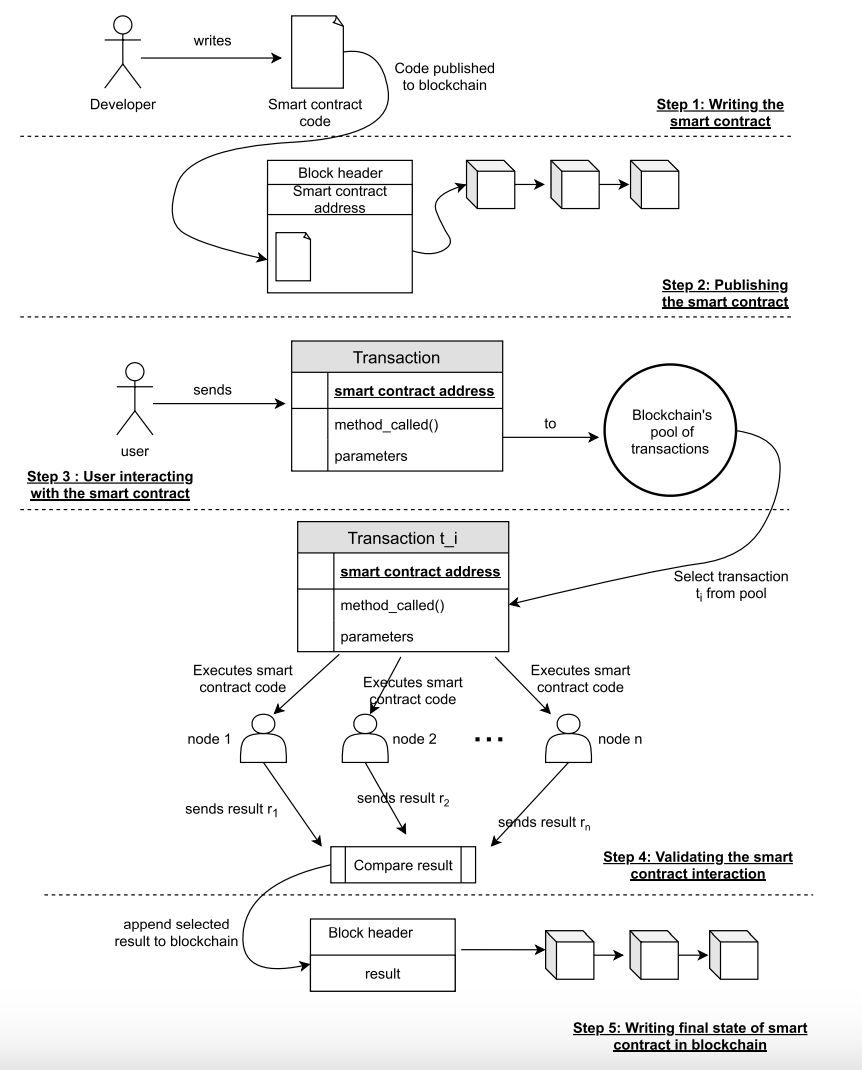
\includegraphics[height = 0.9 \textwidth,width=0.8\textwidth]{overview of smart contract.png}
  \caption{Overview of smart contracts.}
  \label{fig:Overview of smart contracts}
\end{figure}

The process of deploying a smart contract on a blockchain platform typically involves the following steps:

\begin{enumerate}
    \item Developers write the smart contract logic using a supported programming language for the target blockchain platform. They then compile the source code using a specific compiler provided by the platform to obtain a byte code representation of the contract.
    \item The compiled byte code is published to the blockchain platform, where it is stored on the blockchain. Depending on the platform, the smart contract program may be read-only or modifiable. For example, Ethereum does not allow modifications to smart contracts \cite{ethereum_whitepaper}, while EOSIO allows overwriting by uploading new byte code \cite{eosio_cleos}. If the contract is read-only, developers need to publish a new version to provide updates. The initial state of the smart contract represents the initial values of its internal variables.
    \item Access to a published smart contract depends on the blockchain platform. In Ethereum \cite{ethereum_whitepaper} and Neo \cite{neocontract_whitepaper}, the platform provides an address that developers can use to interact with the contract. In EOSIO \cite{eosio_api}, the contract is published to a previously created account, and the account's identifier is used for access. Once users obtain the address or identifier, they can send transactions to the contract, specifying the desired function and its arguments. If required, the transaction may include an amount of platform currency to initiate the function's execution. The transaction is stored in the platform's transaction pool for execution and validation.
    Step 3 in Figure \ref{fig:Overview of smart contracts} is based on the functioning
of \cite{ethereum_whitepaper}\cite{neocontract_whitepaper}.
    \item From the transaction pool, the blockchain platform selects a set of transactions to be executed and validated. During the execution phase, the specified functions in the transactions are executed by a set of nodes. In the validation phase, the nodes compare their results and reach a consensus on the valid result according to the chosen consensus protocol. For example, in a  \ac{BFT} \cite{pease_reaching_1980} consensus protocol, a certain number of nodes are selected to execute and validate transactions, and the result agreed upon by the majority of nodes is considered valid. Other consensus protocols include proof-based consensus, where each node must provide a valid proof of execution \cite{nguyen_survey_2018}, and hybrid protocols that combine \ac{BFT} and proof-based mechanisms \cite{pass_hybrid_2017}\cite{wu_hybrid_2020}.
    \item Once the valid result is determined, it is inserted into a block that is appended to the blockchain. Additionally, the initial state of each smart contract specified in the executed transactions is updated. If a validated transaction modified the internal variables of a smart contract, the new values become the initial values for future transactions involving the contract.
\end{enumerate}

\subsubsection{Source Code and Bytecode}
    
    The code for a smart contract is commonly written in Solidity, a language that shares similarities with JavaScript in terms of syntax. Solidity smart contracts have a structure resembling that of a class in object-oriented programming. Figure \ref{fig:An example of a smart contract written in Solidity} provides an illustrative example. Comparable to the Java compiler, the Solidity compiler generates bytecode from the source code, which is then executed by the \ac{EVM}. The Ethereum bytecode consists of various opcodes, which are low-level instructions. It is essential to note that only the bytecode of a smart contract is stored in Ethereum. Additional information regarding Solidity and its bytecode format can be found in the official Solidity documentation \cite{solidity_doc}.
    
 \begin{figure}[H]
 \centering
  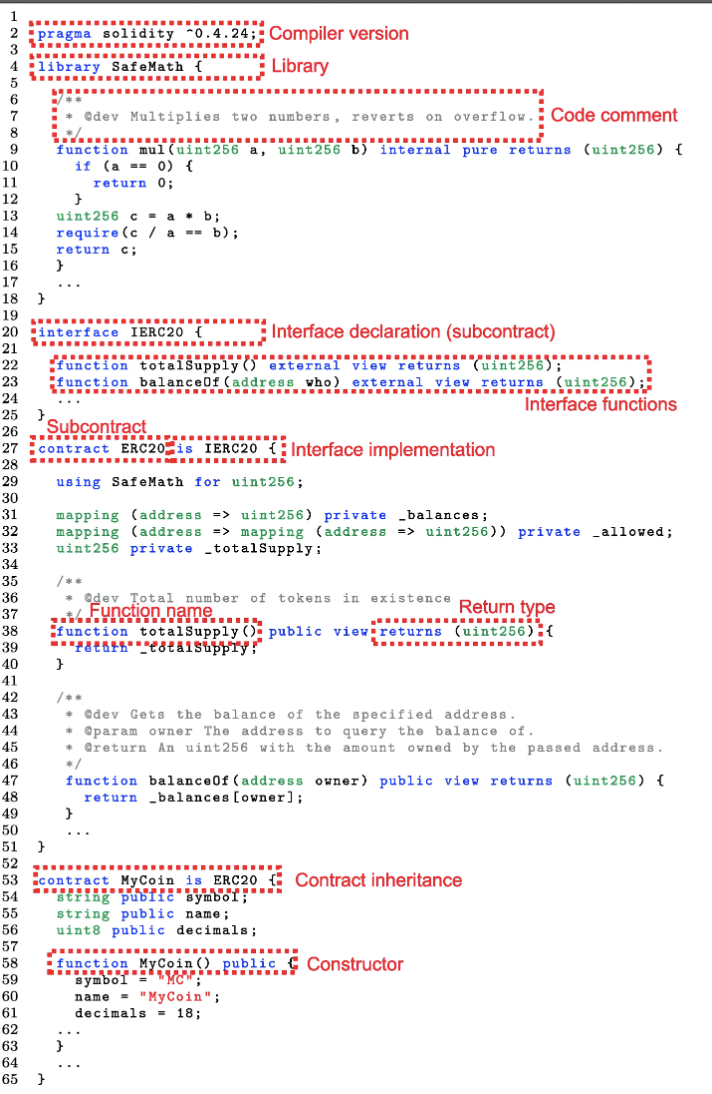
\includegraphics[height=0.7\textwidth  ,width=0.5\textwidth]{smart contract code.png}
  \caption{An example of a smart contract written in Solidity.}
  \label{fig:An example of a smart contract written in Solidity}
\end{figure}

\subsubsection{Subcontracts and Libraries}

In order to enable separation of concerns, the Solidity language provides subcontracts and libraries constructs. Similarly to nested classes (as in object-oriented programming), subcontracts and libraries have each a specific purpose. Subcontracts enable developers to establish object-oriented relationships between contracts, such as inheritance and interface implementation. Libraries often provide a set of utility methods that are mindful of corner-cases or optimize processing time (e.g., a library to perform mathematical operations without incurring into underflows and underflows). In the example depicted in Figure \ref{fig:An example of a smart contract written in Solidity}, there are two subcontracts (ERC20 and MyCoin) and two libraries (SafeMath and VectorSum).

\subsection{Platforms}

Bitcoin is recognized as one of the prominent blockchain technology products, driving ongoing advancements in research and technology commercialization. It serves as the groundbreaking catalyst for the emergence of blockchain 1.0 and the development of cryptocurrency. This technology exhibits key characteristics such as decentralization, resilience to damage, anonymity, and auditing capabilities \cite{dmitry_roschin_blockchain}. Bitcoin operates on the foundation of the blockchain system. However, when it comes to implementing intricate contract logic, Bitcoin encounters a limitation. Due to the constraints of the Bitcoin scripting language, which encompasses a total of 256 instructions (with 15 currently disabled and 75 reserved), writing complex contract logic becomes impractical. Consequently, Bitcoin can be regarded merely as a rudimentary prototype of a smart contract. On the other hand, continuous efforts are being made to enhance smart contract functionality. Among the platforms focusing on this area is Ethereum. Ethereum was developed to address the deficiencies of the Bitcoin platform. It revolves around the central concept of executing user-defined programs on the blockchain, enabling the creation of sophisticated custom smart contracts using a Turing-complete programming language \cite{shuai_smart_contract}.

In the development of Ethereum, the Ethereum smart contract code is written in bytecode language based on the stack that runs on the  \ac{EVM} \cite{everett_kevm}\cite{ahmed_hawk}. The high-level languages used in Ethereum development are Solidity1 and Serpent2 \cite{everett_kevm}. After that, the program code is compiled into \ac{EVM} bytecode to run. With complex smart contract logic blockchain technology implemented, currently, Ethereum is the most popular platform for developing smart contracts; then, Ethereum is marked as the developer of blockchain technology which is known as Blockchain 2.0 \cite{imran_mastering_blockchain}. As part of Ethereum, Hyperledger Fabric, Corda, and BigchainDB are several platforms that can be used to develop smart contracts \cite{khaled_blockchain_ai}.
One of the advantages of smart contracts is the implementation of protocols that work by consensus \cite{christian_smart_contract_lifecycle}\cite{massimo_smart_contract_analysis}. Smart contracts will work by encoding predetermined rules and carry out related operations when the agreed provisions have been fulfilled \cite{pierluigi_smart_contracts}. Smart contract implementations can be used in a variety of domains including smart assets \cite{steve_cryptocurrencies_smart_contracts} (e.g., Slock.it3, a German company that uses Ethereum-based smart contracts for leasing, selling, or sharing other transaction activities without the involvement of intermediaries) \cite{steve_cryptocurrencies_smart_contracts}. In addition, the implementation of smart contracts has been used in the implementation of self-government or autonomous arrangements (for example, digital property management such as ujomusic4, e-voting, and supply chain) \cite{natalie_blockchain_media_sector}.


\subsubsection{1. \ac{eGov-DAO}}
  
        One application of blockchain and smart contracts in the government sector is \ac{eGov-DAO}. \ac{eGov-DAO} serves as a framework for smart contracts that enables the provision of e-government services through an automated and efficient system. Its integration ensures transparent service delivery \cite{nour2018egovdao}. The primary purpose of \ac{eGov-DAO} is to facilitate real-time monitoring and analysis of government services while upholding principles such as transparency, accountability, and provision. A significant advantage of this system is its ability to improve the management of national resources \cite{nour2018egovdao}. By maintaining comprehensive audit records, \ac{eGov-DAO} ensures transparency in court proceedings involving relevant parties. The user-friendly design of \ac{eGov-DAO} minimizes the need for extensive user training \cite{nour2018egovdao}.

    The implementation of \ac{eGov-DAO} is particularly beneficial in government contracts, which involve agreements between the government and vendors that are publicly recorded \cite{nour2018egovdao}. The previous system exhibited several weaknesses, including inefficient allocation of contracts and deals that required extensive interaction between institutions, leading to excessive human labor \cite{mark2004contracting}. Furthermore, while the government invested significant human and financial resources in providing excellent services, it resulted in a lack of transparency in government administration and inefficient performance. Smart contracts offer a solution to enhance transparency, trust, cost reduction, and process simplification.

    The \ac{eGov-DAO} framework is a versatile blockchain framework applicable to government contract policies. It was specifically developed with the United States Small Business Administration policy in mind \cite{nour2018egovdao}. The framework's initial phase involves explaining smart contract and blockchain applications in the context of US contracts. It then introduces contract allocation rules mandated by the Small Business Administration policy, and the \ac{DAO} framework incorporates these requirements and governs the allocation process within the smart contract. \ac{eGov-DAO} defines system-related parties, system user activities, and establishes a model for the primary contract process. The final phase of \ac{eGov-DAO} involves validating the agreed-upon rules within the smart contract \cite{nour2018egovdao}.

\subsubsection{2. Manticore}

Manticore is a framework based on blockchain technology that employs a smart contract approach for symbolic execution in binary analysis. It is utilized by Trail of Bits and \ac{DARPA} \ac{CGC} as a symbiotic code testing solution for code assessment and program analysis. One of Manticore's strengths lies in dynamic symbolic execution, which involves exploring the semantic distance of program code. This analysis technique traverses each path, considering all code, and employs dynamic symbolic execution principles. This process entails identifying path predicates and setting constraints for program testing. Despite its advantages, Manticore has not been widely adopted in the industry due to the lack of a flexible and user-friendly tool. Furthermore, the existing framework is closely tied to the traditional execution model, limiting symbolic execution to an alternative technique, such as seen in the Ethereum platform \cite{mossberg2019manticore}.

Manticore’s design is highly flexible and supports both
traditional computing environments (x86/64, ARM) and exotic
ones, such as the Ethereum platform. To our knowledge,
it is the only symbolic execution framework that caters to
such different environments. It is also simple, extensible, and
as self-contained as possible, avoiding unwarranted external
dependencies. Figure \ref{fig:Manticore overview} shows Manticore’s architecture. The primary
components are the Core Engine and Native and Ethereum
Execution Modules. Secondary components include the  \ac{SMT-LIB} module, Event System,
and API.

\begin{figure}[H]
 \centering
  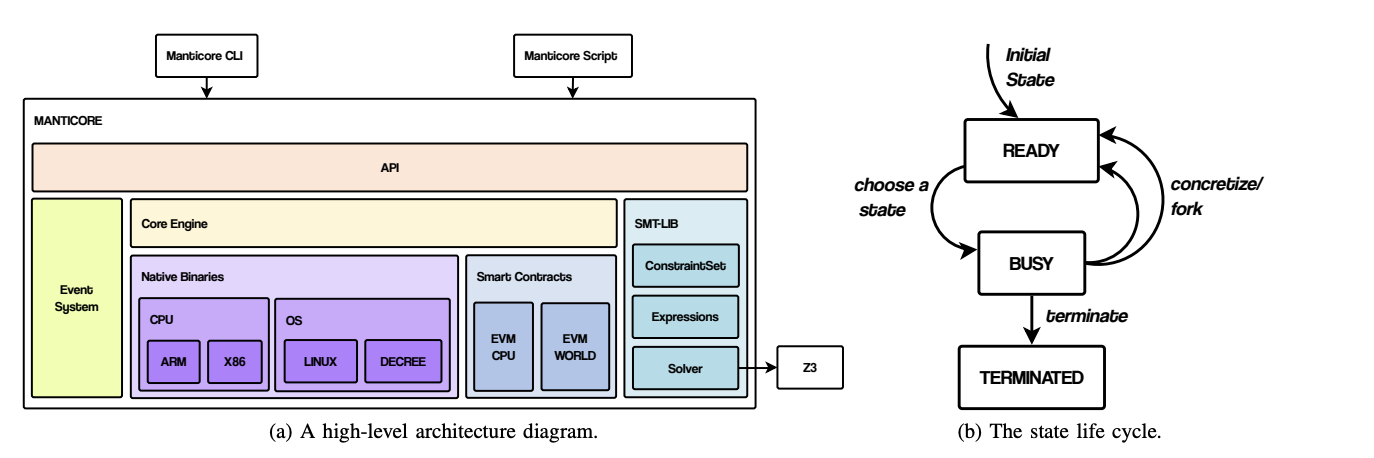
\includegraphics[width=0.8\textwidth]{manitcore overview.png}
  \caption{Manticore overview.}
  \label{fig:Manticore overview}
\end{figure}

The primary function of Manticore is to serve as a technology for program testing using a symbolic execution analysis approach. It can be employed for symbolic execution on various execution platforms. In terms of testing program code, Manticore demonstrates comparable performance to other standard symbolic execution tools, providing an average code coverage of 66\% specifically for smart contracts \cite{mossberg2019manticore}.
        
Over the past decade, symbolic execution has witnessed significant development and research interest, resulting in the creation of notable symbolic execution tools like KLEE, which is the foremost and widely adopted example of symbolic execution today. Additionally, several symbolic execution frameworks are currently under development, including Angr, Triton, binsec, and miasm. These platforms are renowned in the field of binary analysis and offer extensive symbolic execution functionality that finds wide application in commercial software auditing \cite{mossberg2019manticore}.

\subsubsection{3. \ac{SODA}}

    Current methods for safeguarding smart contracts can be broadly classified into two categories: offline and online. Offline approaches involve analyzing the code of smart contracts for potential vulnerabilities, checking for accuracy, reverse engineering bytecode, and detecting malicious code. However, offline methods have limitations as they lack runtime information, which can result in the failure to detect and remove all vulnerabilities. On the other hand, online approaches are intended to detect attacks targeting smart contracts or protect them from attacks after deployment. These approaches fall into two categories: those that add protection code into the source/bytecode of smart contracts and those that add protection code into the runtime of smart contracts (such as \ac{EVM}). However, these methods have limitations such as size restrictions and gas mechanisms for bytecode protection, and they can be resource-intensive, leading to potential detection failures.

    Smart contracts have attracted the attention of attackers due to their potential for significant cost savings. However, existing offline methods for identifying vulnerabilities or verifying smart contracts lack the capability to detect online attacks in real-time. Moreover, current online approaches are limited in their focus on specific attack types and cannot be easily extended to detect new forms of attacks. Developing a new online detection system for smart contracts from scratch is a time-consuming task that requires a deep understanding of blockchain internals, making the implementation of new attack detection mechanisms challenging \cite{chen2020soda}.


As shown in Figure \ref{fig:SODA architecture}, \ac{SODA} is integrated into a full node of
any \ac{EVM}-compatible blockchain, because only a full node can
mine blocks. It separates the information collection and attack
detection with layered design for the ease of developing detection apps. More precisely, \ac{SODA} uses three modules, namely
block collector, trans collector and ins collector, to collect
the primitive information of blocks, transactions, and executed
\ac{EVM} instructions, respectively, from the smart contract layer,
the consensus layer and the data layer of a full node. Note that
\ac{EVM} serves the data, consensus, and application layers \cite{bez2019scalability},
where the data layer contains the defined data structures and
the data types (e.g., account, transactions), the consensus layer
regulates how nodes reach consensus, and the smart contract
layer stores smart contracts \cite{bez2019scalability}.

\begin{figure}[H]
 \centering
  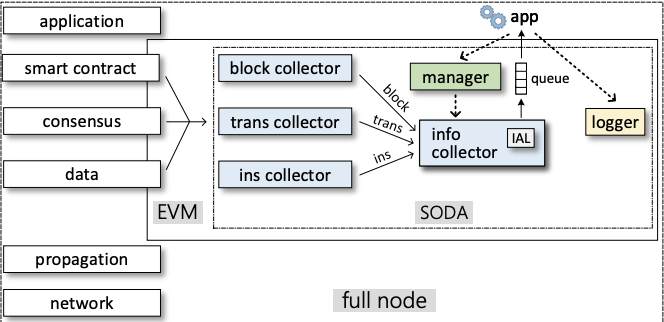
\includegraphics[width=0.8\textwidth]{SODA Architec.png}
   \caption{SODA architecture.}
  \label{fig:SODA architecture}
\end{figure}

Introducing \ac{SODA}, a novel and comprehensive online detection framework compatible with all blockchains supporting the \ac{EVM}. \ac{SODA} sets itself apart from existing online approaches by offering enhanced capabilities, efficiency, and compatibility. Firstly, \ac{SODA} provides users with a user-friendly platform for developing various attack detection applications, separating information gathering and attack detection through a layered design. At a higher layer, \ac{SODA} presents a unified interface for creating diverse attack detection applications. At a lower level, \ac{SODA} instructs the \ac{EVM} to collect essential primitive information necessary for detecting a range of attacks and constructs 11 types of structural information to simplify application development. Leveraging \ac{SODA}, users can swiftly develop new applications with minimal code modifications to the \ac{EVM}. Secondly, \ac{SODA} focuses on efficiency by implementing on-demand information retrieval to minimize additional costs associated with information gathering. Additionally, it employs dynamic linking to eliminate the overhead from inter-process communication. This design enables users to develop detection applications using any programming language capable of generating dynamic link libraries. Thirdly, as more blockchains adopt the \ac{EVM} as the smart contract runtime, \ac{EVM} offers seamless migration without requiring application modifications. To date, eight detection applications have been developed using \ac{SODA} to identify attacks exploiting major vulnerabilities in smart contracts. \ac{SODA} has been integrated into three popular blockchains: Ethereum, Expanse, and Wanchain. Extensive experimental results demonstrate the effectiveness and efficiency of \ac{SODA} in various detection applications \cite{chen2020soda}.


\subsection{Ethereum}
Ethereum is a software platform built on blockchain technology that enables the creation and execution of smart contracts and  \ac{DApps}. It serves as the foundation for a virtual currency called Ether. Smart contracts on Ethereum are defined using a Turing-complete programming language, allowing the creation and execution of programs on the blockchain. Ethereum operates using accounts and their balances, which change through state transitions. The state represents the current balances of all accounts and additional data, and it is encoded and maintained by accounts in a separate data structure called a Merkle Patricia tree. Accounts on Ethereum are pseudonymous, providing a level of anonymity, and can be linked to one or more addresses.
There are two types of accounts: externally owned accounts, controlled by individuals who possess private keys for transactions, and contract accounts, controlled by smart contract code. Contract accounts function as cyber-entities with their own balances and can be triggered by transactions from external accounts or other contracts. When triggered, the specified code in the contract is executed, which can generate further transactions. The presence of these smart contracts allows developers to use Ethereum as a versatile framework for creating \ac{DApps}.

Figure \ref{fig:Ethereum Blockchain} presents an overview of Ethereum blockchain, which
consists of the following layers from bottom to top: peer,
blockchain, smart contract, and token.
\begin{figure}[H]
 \centering
  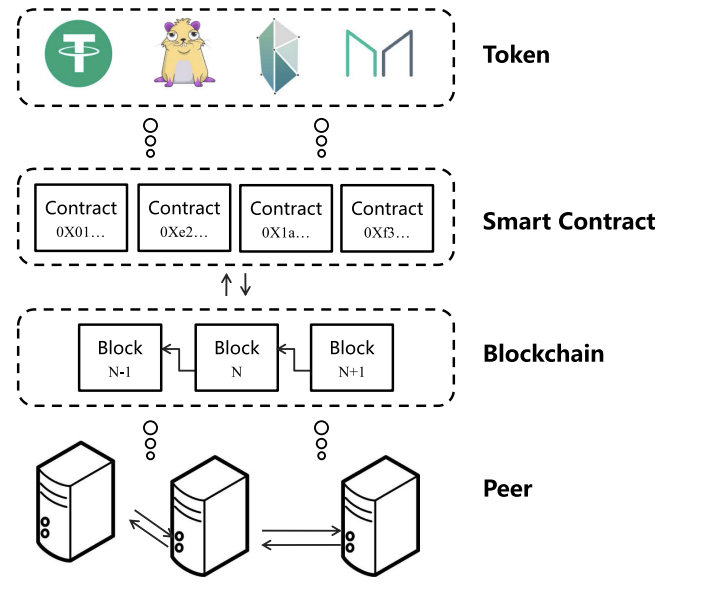
\includegraphics[width=0.8\textwidth]{Overview of Ethereum.png}
  \caption{Ethereum Blockchain.}
  \label{fig:Ethereum Blockchain}
\end{figure}

Ether is the cryptocurrency used within the Ethereum blockchain. It serves as fuel for operating distributed applications, making payments to other accounts or machines executing requested operations. Ether enables the execution of \ac{DApps}, facilitates the use of smart contracts, allows the generation of tokens during \ac{ICOs} for cryptocurrency-based funding, and supports standard peer-to-peer payments. This is why Ethereum is often referred to as "programmable money."

\subsubsection{Ethereum Virtual Machine (EVM)}
In Ethereum, the execution of a smart contract takes place within a specialized environment known as the \ac{EVM}. The \ac{EVM} interacts with the states stored as key-value pairs, based on the actions specified in the smart contract. Figure \ref{fig:EVM role} illustrates the
typical Ethereum transaction execution flow from Block N 
to \ac{EVM} through Blockchain peer.
\begin{figure}[H]
 \centering
  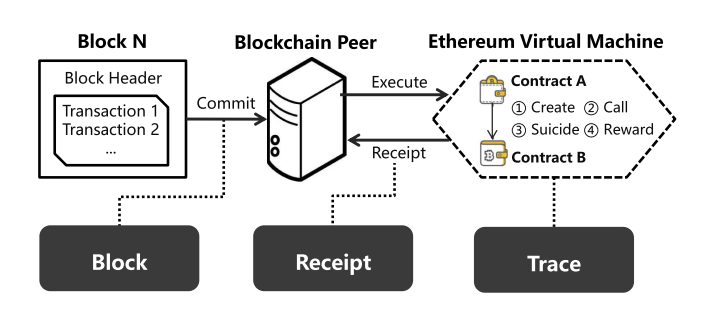
\includegraphics[width=0.8\textwidth]{EVM.png}
  \caption{EVM role in blockchain.}
  \label{fig:EVM role}
\end{figure}

During the execution of a contract, a miner utilizes "Gas" as a unit to measure the consumption of the contract. The contract user is charged based on the "GasUsed" and "GasPrice" parameters. If users offer a higher "GasPrice" to the miner, the contract will execute more quickly. Once the transactions or operations are completed, the \ac{EVM} generates a hash value representing the state and records it in the blockchain.Consequently, it can be observed that smart contracts in Ethereum are not directly stored on the blockchain itself. Instead, they are essentially stored within the states that have been manipulated by the blockchain.


\subsection{Canister}

A smart contract is like a computer program that runs on a blockchain. On the Internet Computer, a smart contract takes the form of a canister, which combines the program itself with its associated data. Each canister is hosted on a specific subnet of the Internet Computer. One advantage of canisters is their ability to execute concurrently, meaning multiple canisters can run simultaneously. They can also communicate with each other within and across subnets by sending asynchronous messages, and this communication is non-blocking, allowing for virtually unlimited scalability.

Canisters are more powerful than smart contracts on other blockchains as they can:

\begin{itemize}
    \item serve a user interface directly to any web browser.
    \item hold gigabytes of memory for a low fee.
    \item perform substantial amounts of computation at a low cost.
    \item pay for their own computation (reverse gas model).
\end{itemize}


The code of a canister is composed of a WebAssembly (Wasm) module, which is a type of module used in web development. The state of a canister includes the standard heap of the Wasm module, along with stable memory as shown in Figure \ref{fig:Canister}. Stable memory is a special type of memory that plays a crucial role in the life cycle of a canister.

\begin{figure}[H]
 \centering
  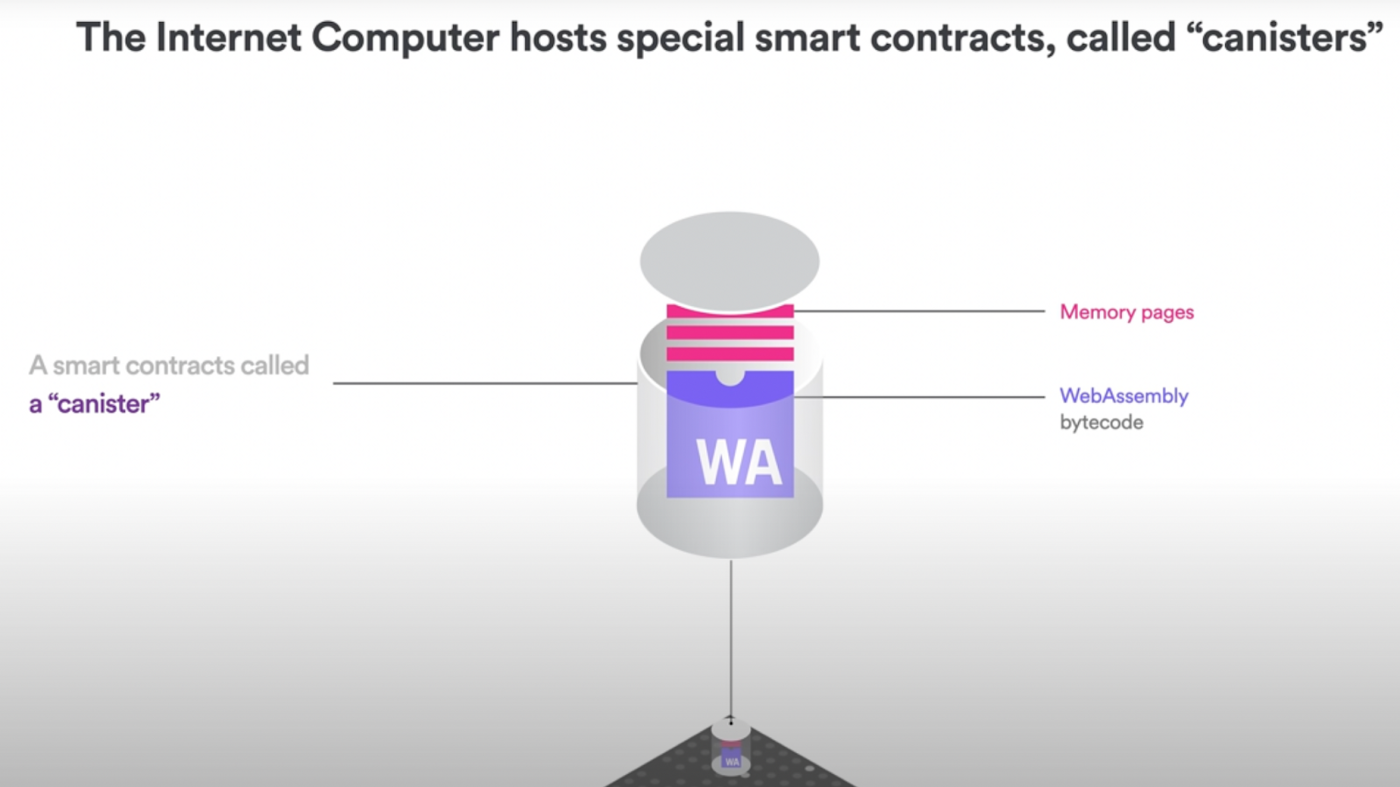
\includegraphics[width=0.5\textwidth]{canister overview.png}
  \caption{Overview of Canister.}
  \label{fig:Canister}
\end{figure}

Canisters on the Internet Computer have endpoints that can be accessed by other canisters as well as external parties like browsers or mobile apps. These endpoints come in two types: updates and queries. Updates are calls that have the ability to modify the state of a canister, while queries are limited to reading from the state. To simplify, think of updates as used for writing to the canister's state, and queries as used for reading from that state.

\subsubsection{How Canister Work}

Canisters on the Internet Computer operate in a manner similar to actors in the actor-based concurrency model. Each canister's code runs on a single thread and is completely isolated from other canisters. Canisters communicate with each other using asynchronous messaging. When a canister receives a message, it has the ability to modify its own state, send messages to other canisters, and even create new canisters. Unlike the traditional actor model, communication between canisters is two-way. Canister messages can be either requests or replies. When a request is sent, the \ac{IC} keeps a record of a callback function to be executed when the receiving canister sends back a response. In cases where the \ac{IC} determines that the receiving canister cannot respond, the system generates a response on behalf of the canister.

Another interesting aspect of the canister-based model is the interaction between message processing and canister trapping. While processing a request, a canister may send requests to other canisters and wait for some or all of the replies before generating a response to the original request. In the event that a canister encounters an issue or exception, it enters a trapped state, and its state is rolled back to the point immediately after it made the last outgoing call.

\subsubsection{Canister Controllers}
Canisters are supervised by controllers, which can be either users or other canisters. The management structure of canisters can take different forms: centralized (when controllers involve a centralized entity), decentralized (when the controller is a \ac{DAO}), or even non-existent, in which case the canister is an immutable smart contract. Controllers are responsible for deploying and maintaining canisters on the \ac{IC}, and they possess the authority to perform management operations on the canisters. Common operations include deploying a canister smart contract to the \ac{IC}, as well as starting and stopping canisters. Controllers have the ability to modify canister parameters, such as adding or removing controllers and adjusting the freezing threshold.

Controllers can update the code running on canisters by submitting a new \ac{Wasm} module to replace the older one. By default, updating the \ac{Wasm} module erases the content of the \ac{Wasm} memory, but the data stored in stable memory remains unchanged. The \ac{IC} provides an upgrade mechanism that executes three actions atomically: serializing the \ac{Wasm} memory of the canister and storing it in stable memory, installing the new \ac{Wasm} code, and then deserializing the content from stable memory. However, a canister can ensure that data requiring persistence across upgrades is always stored in stable memory, simplifying the upgrade process significantly.

\subsubsection{Canister behavior remains consistent.}
Controllers are responsible for deploying and managing canister smart contracts. The level of decentralization of a controller can vary, ranging from an individual or a team of people to being managed by the \ac{NNS} \cite{InternetComputerNNS} or another type of on-chain \ac{DAO}. Controllers have the ability to modify the code of the canisters they control, making canister code mutable unlike traditional smart contracts on other blockchains. Additionally, controllers have complete control over the assets held by the canisters, such as ICP tokens or Bitcoins. This flexibility brings canisters closer to conventional software and enables them to be used in a wide range of applications where the logic of the software needs to be modified as required.

However, in critical applications like those used in \ac{DeFi}, centralized mutability can introduce risks. There is a possibility that a controller could maliciously modify a canister to steal assets. To address this concern, developers have several options available to them to verifiably decentralize the control of canister mutations.

\section{Decentralized Applications (DApp)}

In simpler terms, the blockchain can be understood as a distributed system that enables applications to operate on multiple nodes. Unlike centralized systems, blockchains function based on decentralized consensus models, which means that applications on blockchains are \ac{DApps}. \ac{DApps} are a special type of software where the control over application execution is not held by a single entity. Previously, \ac{DApps} were commonly associated with applications running on a \ac{P2P} network of computers rather than a single central computer. Examples of popular \ac{DApps} include BitTorrent for file sharing, BitMessage for instant messaging, and Popcorn Time for video streaming.

By utilizing smart contracts, blockchains provide a flexible approach to computing, allowing the development of \ac{DApps} for various application scenarios. For example, the Ethereum blockchain offers Turing-complete smart contracts that enable developers to create versatile programs. Consequently, as the popularity of blockchains continues to grow, a wide range of blockchain-based \ac{DApps} have emerged and found applications in diverse domains. According to a recent report, the Ethereum \ac{DApps} market, which is the largest blockchain-based \ac{DApps} market, has reached a valuation in the billions of dollars as of January 2019 \cite{abdulhakeem2021powered}.

In other words,
an ideal blockchain application or service should be operable
without any human intervention, which forms a \ac{DAO}. A \ac{DAO} is an
organization that is run through rules encoded as smart contracts running on the blockchain. Due to its autonomous and
automatic nature, a \ac{DAO}’s cost and profit are shared by all
participants by simply recording all activities into the blocks.
In fact, Bitcoin, the most classic blockchain system, is an
example of a \ac{DAO}. According to the definition of \ac{DApps}
in \cite{raval2016decentralized}, \ac{DApps} are characterized by four properties as follow:
\begin{itemize}
    \item[--] \textit{Open Source}: Due to the trusted nature of blockchain,
\ac{DApps} need to make their codes open source, so that
audits from third parties become possible.
    \item[--] \textit{Internal Cryptocurrency Support}: Internal currency is
the vehicle that runs the ecosystem for a particular
\ac{DApps}. With tokens, it is feasible for a \ac{DApps} to quantify
all credits and transactions among participants of the
system, including content providers and consumers.
    \item[--] \textit{Decentralized Consensus}: The consensus among decentralized nodes is the foundation of transparency.
    \item[--] \textit{No Central Point of Failure}: A fully decentralized system should have no central point of failure since all components of the applications will be hosted and executed
in the blockchain.
\end{itemize}

 Table \ref{tab:Top 10 Dapps in State of the ÐApps} shows top 10 \ac{DApps} on State of the \ac{DApps}
and their numbers of related transactions from August 2017 to July
2018 respectively.
\begin{table}[H]
\centering
\caption{Top 10 \ac{DApps} in State of the \ac{DApps}}
\begin{tabular}{|c|c|}
\hline
\textbf{Title} & \textbf{Number of Transactions} \\
\hline
ForkDelta & 9,575,884 \\
\hline
IDEX & 3,862,946  \\
\hline
CryptoKitties & 3,130,573  \\
\hline
Bitcoinereum & 1,451,752 \\
\hline
OmiseGO & 1,271,880 \\
\hline
Storj & 769,872 \\
\hline
Ethereum Name Service & 456,702 \\
\hline 
Status & 407,946 \\
\hline
PoWH 3D & 327,353 \\
\hline
Ether Goo & 312,140 \\ \hline
\end{tabular}
\label{tab:Top 10 Dapps in State of the ÐApps}
\end{table}
For each \ac{DApps}, the website provides it’s title, description, categories, submit time and smart contract addresses. It summaries
transactions daily and generates sparklines of users, transactions
and volumes. The website marks dapps with categories and badges
(e.g. status), and ranks them by dau (the number of daily active
unique addresses).